\documentclass{article}
\usepackage{graphicx} % new way of doing eps files
\usepackage{listings} % nice code layout
\usepackage[usenames]{color} % color
\usepackage{float}
\definecolor{listinggray}{gray}{0.9}
\definecolor{graphgray}{gray}{0.7}
\definecolor{ans}{rgb}{1,0,0}
\definecolor{blue}{rgb}{0,0,1}
% \Verilog{title}{label}{file}
\newcommand{\Verilog}[3]{
  \lstset{language=Verilog}
  \lstset{backgroundcolor=\color{listinggray},rulecolor=\color{blue}}
  \lstset{linewidth=\textwidth}
  \lstset{commentstyle=\textit, stringstyle=\upshape,showspaces=false}
  \lstset{frame=tb}
  \lstinputlisting[caption={#1},label={#2}]{#3}
}


\author{Jiasen Zhou and Jon Johnston}
\title{Lab 13: Pipelining with Branching or Forwarding}

\begin{document}
\maketitle

\section{Executive Summary}
The purpose of this lab was to add the register buffers between each stage and ultimately to get a barebones pipelined datapath working. The iFetch, iDecode, iExecute, iMemory and iWriteback stages were all connected together with buffers placed at the beginning of each module to ensure data would be passed at the correct time. This pipeline was tested with the 10 test instructions, excluding NOPs added between some instructions. 4 NOPs were added after 6 of the instructions since the datapath did not have data forwarding or hazard detection, so the datapath must wait until the writeback stage to continue operation. After comparing the results of the simulation against the expected results, this lab was successful.


\section{Test Report}
To verify operation of the pipeline, this lab requires 1 test bench.
\begin{enumerate}
	\item Pipeline simulation
\end{enumerate}
\subsection{Pipeline Test Bench}
The Pipeline Test Bench contains:
\begin{enumerate}
	\item Inputs
	\begin{enumerate}
		\item branch\_target - branch address
		\item pc\_src - the control of branch mux
		\item reset - set the current pc to be 0
	\end{enumerate}	
\end{enumerate} 
\pagebreak

\begin{figure}[H]
		\begin{center}
		\caption{Pipeline buffer table.}\label{fig:ert_pipelinebuffer}
		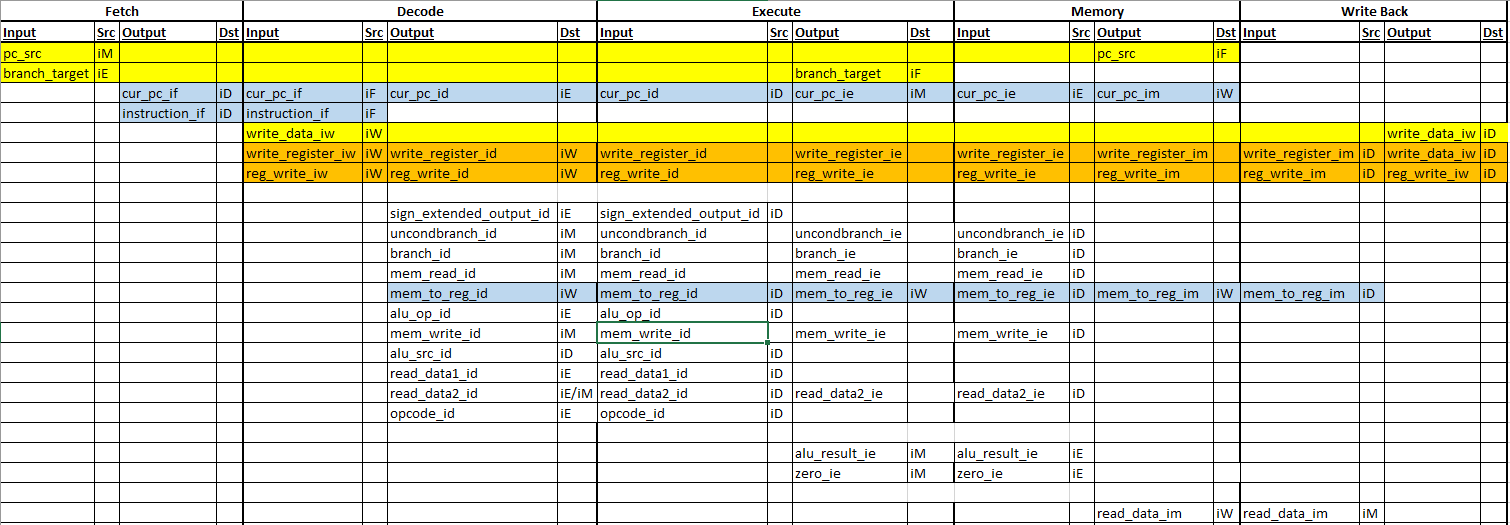
\includegraphics[width=1.0\textwidth]{../images/Lab12_pipelined_datapath_table.png}
	\end{center}
\end{figure}
\begin{figure}[H]
	\begin{center}
		\caption{Expected Results of the pipeline test.}\label{fig:ert_pipelinetest}
		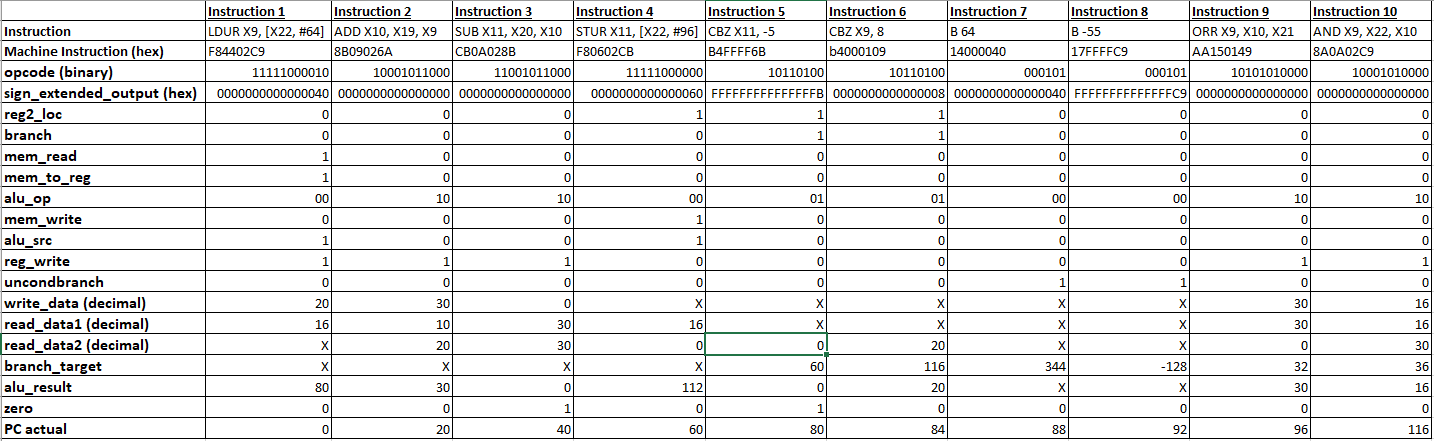
\includegraphics[width=1.0\textwidth]{../images/Lab13_pipeline_table.png}
	\end{center}
\end{figure}

\begin{figure}[H]
	\begin{center}
		\caption{Timing diagram for the pipeline test.}\label{fig:pipelinetest}
		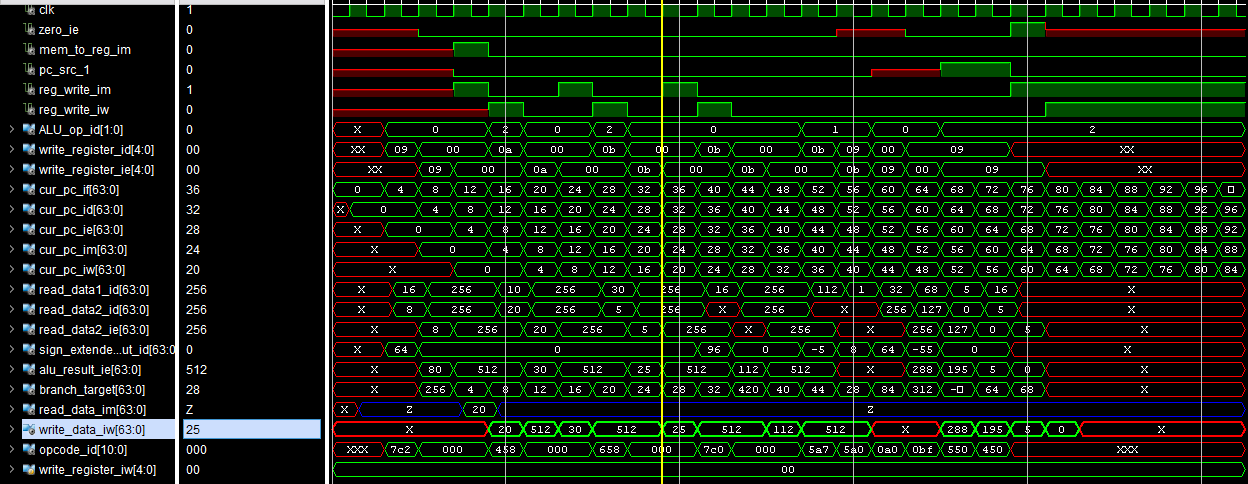
\includegraphics[width=1.0\textwidth]{../images/Lab13_pipeline_timing_diagram.png}
	\end{center}
\end{figure}


\section{Code Appendix}
% The code appendix should include the test bench code and module code for this lab.
\Verilog{Verilog code of pipeline.}{code:pipelinetest}{../code/2_decode/pipeline_datapath.v}

\end{document} 